\section{3-lambda Model} 
\label{sec:met}
%As mentioned in the introduction, the model is based on the assumption that one-step of the network's growth is one interaction. Both new and existing nodes are involved in the interaction and after the interaction there are edges between all involved pairs of nodes. Some (or all) of these edges between pairs of involved nodes could exist before the interaction. The model is inherently temporal, since with each node or edge we can associate the list of interactions in which they participated during the growth of the network (list of interactions is a list of steps of the growth in the order in which interactions took place). It is further assumed that neither nodes nor edges age, so they are not removed during the growth of the network. From this perspective, the model is growing.

\begin{figure*}[ht]
\centering
 \begin{subfigure}{17em}
  \centering
	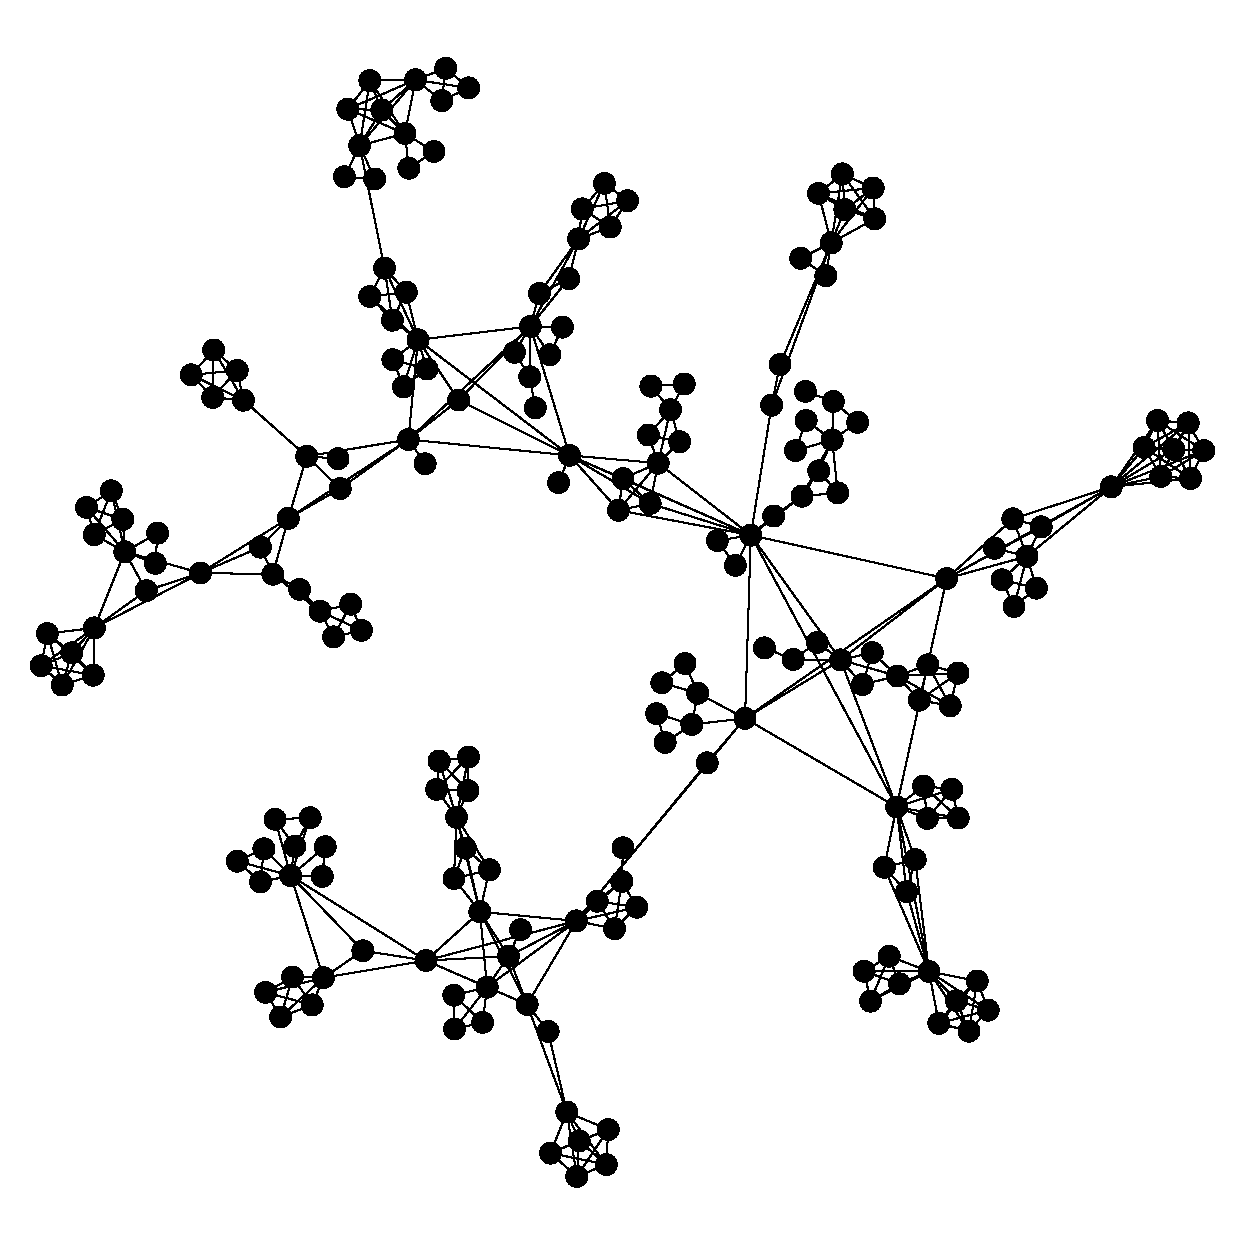
\includegraphics[width = 16em]{figures/200-0-3-0}
\caption{$\lambda_1$ = 0, $\lambda_2$ = 3, $\lambda_3$ = 0}
\label{fig:lambda2net}
 \end{subfigure}
 \begin{subfigure}{17em}
	\centering
		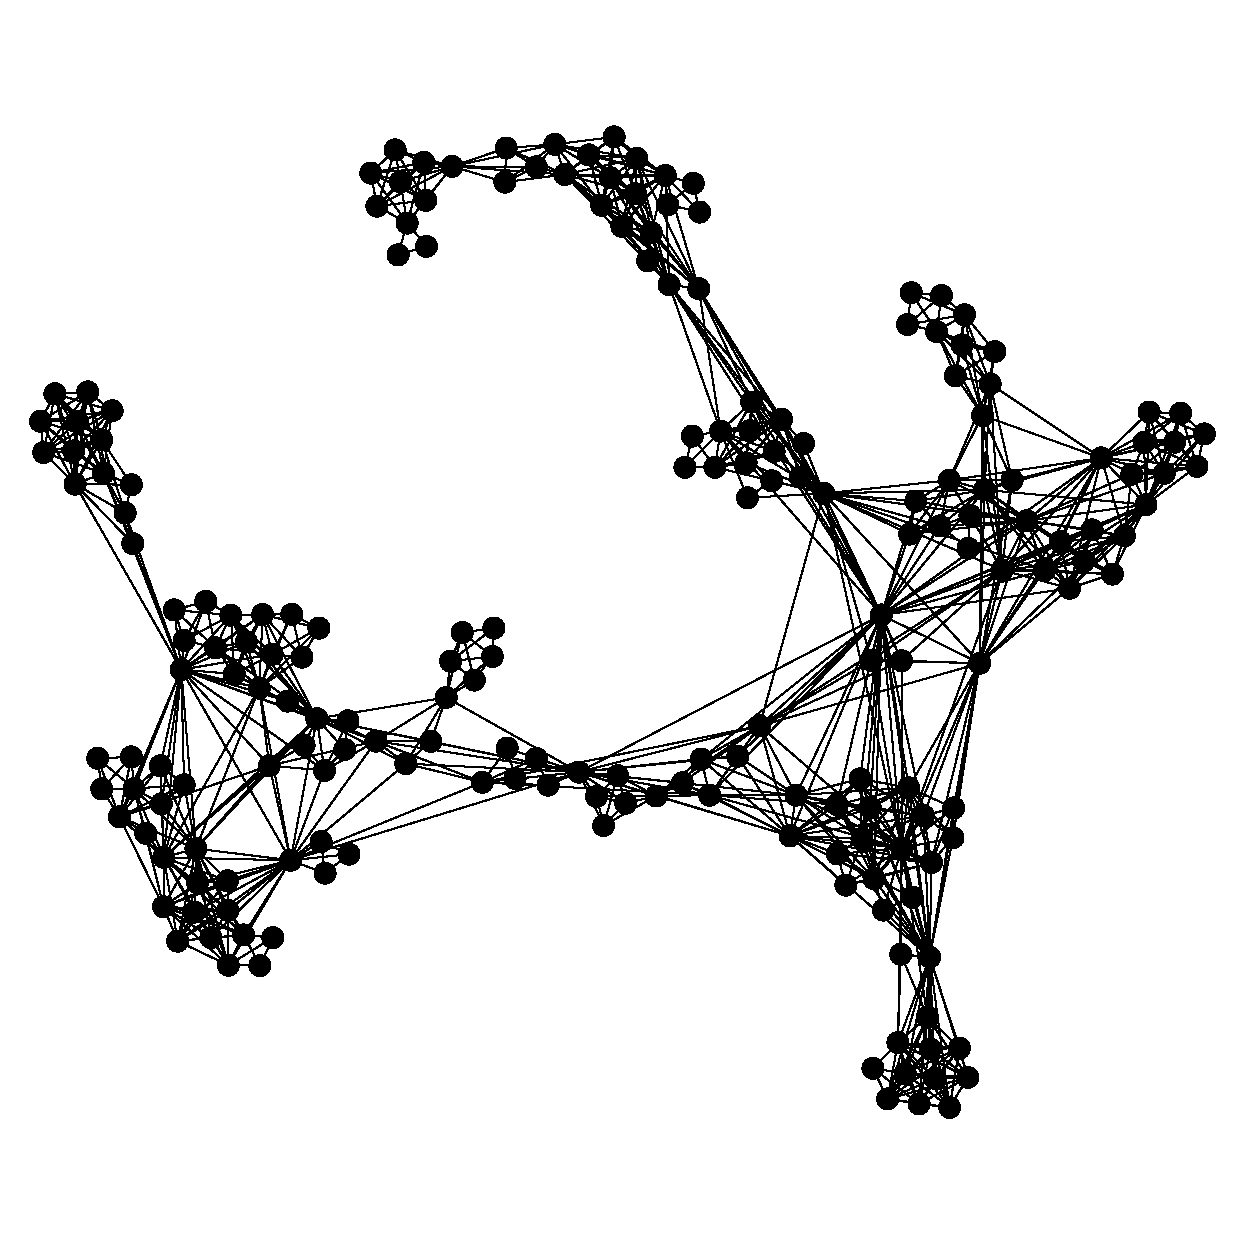
\includegraphics[width =16em]{figures/200-2-3-0}
		\caption{$\lambda_1$ = 2, $\lambda_2$ = 3, $\lambda_3$ = 0}
		\label{fig:lambda1net}
  \end{subfigure}
  \begin{subfigure}[ht]{17em}
		\centering
			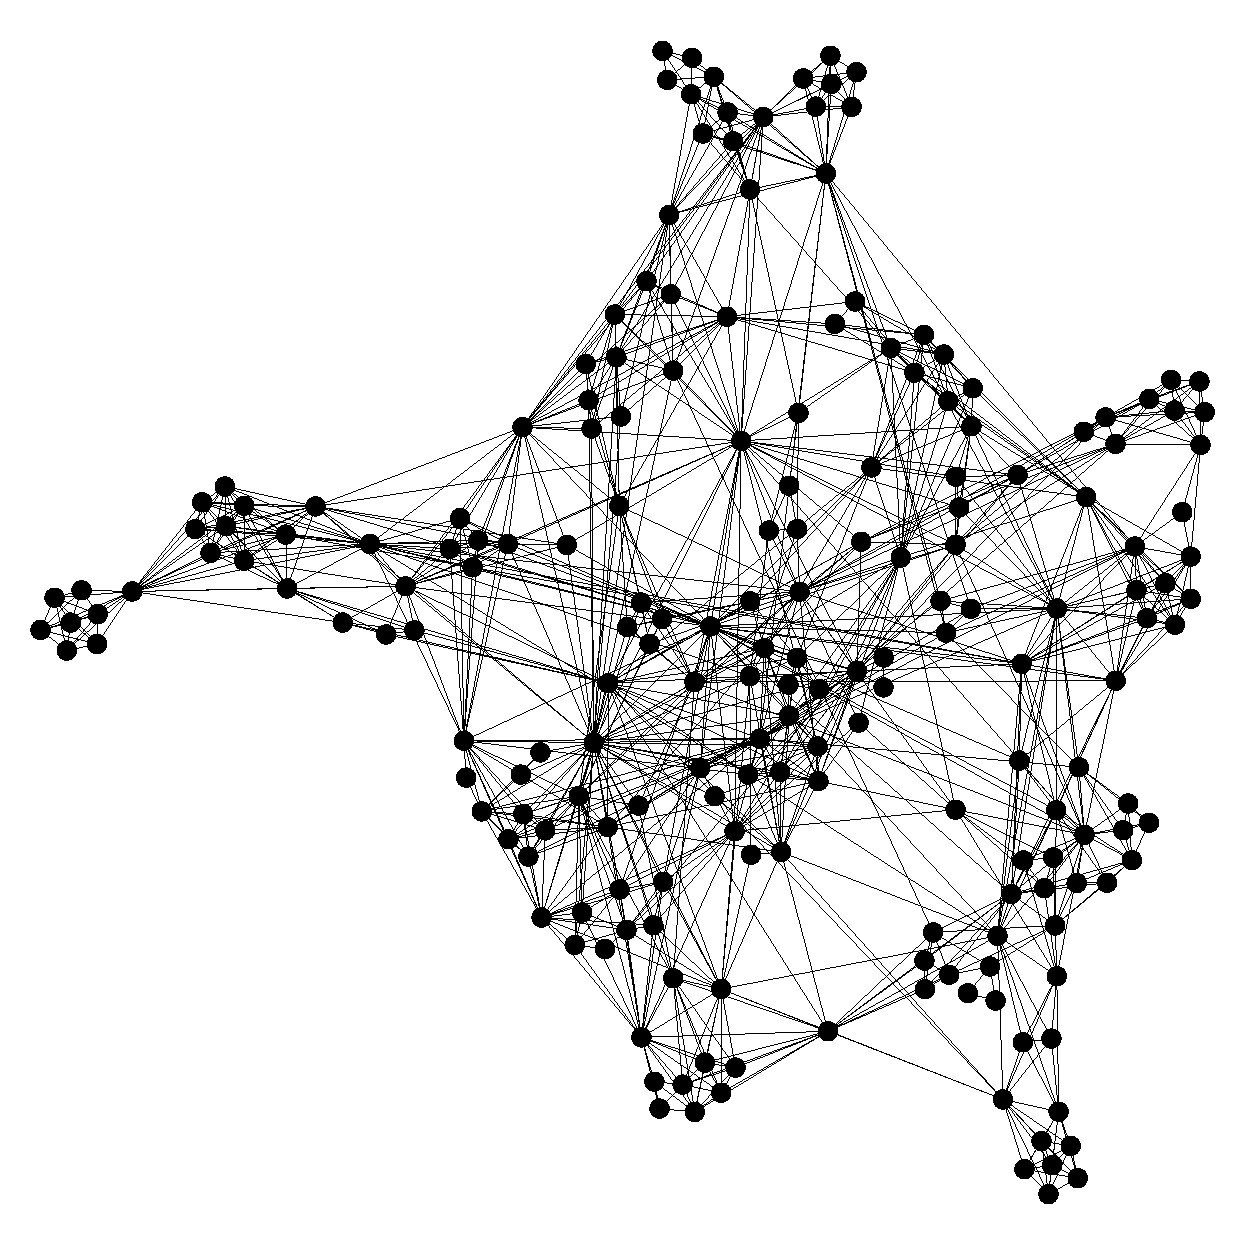
\includegraphics[width =16em]{figures/200-2-3-05}
			\caption{$\lambda_1$ = 2, $\lambda_2$ = 3, $\lambda_3$ = 0.5}
			\label{fig:lambda3net}
  \end{subfigure}
	\caption{3-lambda model: generated networks with $200$ nodes}
\label{fig:L3D}
\end{figure*}

As mentioned in the introduction, the model is based on the assumption that one step of the network's growth is one interaction. Both new and existing nodes are involved in the interaction, and after the interaction, there are edges between all involved pairs of nodes. Some (or all) of these edges between pairs of involved nodes could exist before the interaction. The model is inherently temporal since we can associate with each node or edge the list of interactions in which they participated during the growth of the network (the list of interactions is a list of steps of the growth in the order in which the interactions took place). It is further assumed that neither nodes nor edges age, so they are not removed during the growth of the network. From this perspective the model is growing.

In the model, nodes involved in the interaction have four different roles:

\begin{enumerate}
	\item key node of the interaction (proactive)
  \item nodes adjacent to the proactive node (neighbors)
  \item new nodes (newbies)
  \item nodes that are not adjacent to the proactive node (new connections)
\end{enumerate}

It is essential for the model that each interaction always contains exactly one proactive node and may (but doesn't have to) include nodes in three other roles. How many spots will be represented by each of these three roles is selected based on the Poisson distribution with a preselected $\lambda_1$ (neighbors); $\lambda_2$ (newbies); and $\lambda_3$ (new connections). Furthermore, the model assumes that the selection of specific existing nodes for neighbor roles (in the number equal to the maximum number of all neighbors at most) and new connections is random.


%A natural characteristic of the model is that nodes with a higher degree are more likely to participate in the interaction, in which the proactive node has at least one neighbor. Although proactive node of the interaction and its neighbors are being selected at random, high degree node has a greater chance of being selected as neighbor of the proactive node.

A natural characteristic of the model is that nodes with a higher degree are more likely to participate in an interaction in which the proactive node has at least one neighbor. Although a proactive node of the interaction and its neighbors are being selected at random, a high degree node has a greater chance of being selected as a neighbor of the proactive node.


$\lambda_1$, $\lambda_2$ and $\lambda_3$ significantly affect the density of the network. If we assume that a randomly selected interaction has, based on the corresponding distributions, $b$ neighbors of a proactive node, $n$ new nodes and $e$ nodes unconnected to the proactive node, then the number of nodes involved in this interaction (interaction size) is in Equation \ref{eq:xdef} 

\begin{equation} s = 1 + b + n + e \label{eq:xdef}
\end{equation}

and the following applies:

\begin{itemize}
	\item $n$ new nodes, which must connect to a proactive node and each other, is created.
	\item There are $b$ nodes adjacent to the proactive node which must first get connected among each other, then with $e$ nodes that are not adjacent to the proactive node (these edges may already exist prior to the interaction). Finally, they must connect with the new $n$ nodes.
	\item There are $e$ nodes not adjacent to the proactive node, which must get connected with it. Next, they must get connected among each other (these edges may already exist prior to the interaction) and $n$ new nodes.
\end{itemize}

%It follows, that the minimum and the maximum number of new connections (edges) is:

The minimum and the maximum number of new connections (edges) is in Equations \ref{eq:min} and \ref{eq:max}, respectively.

\begin{equation}	MIN = n + e + b \cdot n + e \cdot n + \frac{n \cdot (n - 1)}{2} \label{eq:min}
\end{equation}

\begin{equation} MAX = MIN + e \cdot b + \frac{b \cdot (b - 1)}{2} + \frac{e \cdot (e - 1)}{2} \label{eq:max}
\end{equation}

Thus, if for example we set $b = 2, n = 3, e = 1$ for the interaction, then:

\begin{itemize}
	\item interaction size is $s = 1 + 2 + 3 + 1 = 7$
	\item after the interaction a total of $21$ edges exist between pairs of nodes
	\item $MIN = 3 + 1 + 6 + 3 + 3 = 16$ in the case of $5$ edges existing between pairs of nodes prior to the interaction
	\item $MAX = 10 + 2 + 1 + 0 = 19$ in the case of $2$ edges existing between pairs of nodes prior to the interaction
\end{itemize}

Each of $\lambda_1$, $\lambda_2$ and $\lambda_3$ affects different property of the network generated by 3-lambda model.

%\noindent
%\noindent
%$\lambda_2$ (newbies) defines the growth rate of the network and provides a tree-like network structure, see Fig. \ref{fig:lambda2net}. To construct a network with $N$ nodes requires approximately $N/$$\lambda_2$ interactions.
%
%
%\noindent
%\noindent
%$\lambda_1$ (base/neighbors) constitutes network community structure through local connections of existing neighbors and new nodes, see Fig. \ref{fig:lambda1net}.
%
%\begin{flushright}
%
%\end{flushright}
%
%\noindent
%\noindent
%$\lambda_3$ (new connections) ensures linking of nodes that are not adjacent, thereby linking communities. The consequence is emerging of \textit{nested - core - periphery} network structure, see Fig. \ref{fig:lambda3net}.

\begin{itemize}
	\item $\lambda_2$ (newbies) defines the growth rate of the network and provides a tree-like network structure, see Fig. \ref{fig:lambda2net}. To construct a network with $N$ nodes requires approximately $N/$$\lambda_2$ interactions.
	\item $\lambda_1$ (neighbors) constitutes network community structure through local connections of existing neighbors and new nodes, see Fig. \ref{fig:lambda1net}.
	\item $\lambda_3$ (new connections) ensures linking of nodes that are not adjacent, thereby linking communities. The consequence is emerging of core-periphery network structure, see Fig. \ref{fig:lambda3net}.
\end{itemize}


%Figure \ref{fig:wholenet} shows a network with $1003$ nodes and $5594$ edges generated with parameters $\lambda_1$ = 2, $\lambda_2$ = 3, $\lambda_3$ = 0.5. A total of $347$ interactions took place. The size of nodes and strength of edges correspond to the number of interactions they took part in, the label indicates the order in which nodes were created. The network has a distinct \textit{community} and \textit{nested - core - periphery} structure. Colored $17$ communities were detected  by Louvein[REF!!] method, modularity is $0.683$.
%
%\begin{figure}[h]
%\centering
%\includegraphics[width =\columnwidth]{figures/1000-2-3-05}
%\caption{$\lambda_1$ = 2, $\lambda_2$ = 3, $\lambda_3$ = 0.5; 1003 nodes network}
%\label{fig:wholenet}
%\end{figure}

\subsection{Network Generator}
\label{sec:alg}
The network generator uses a simple algorithm which comes directly from the model description. The only extra step is setting up the initial network state. The model is memory-less, which allows working with an arbitrary initial state. For our generator we chose a complete graph with a number of nodes equal to the round of $(1 + \lambda_1 + \lambda_2 + \lambda_3)$ as the default state. Algorithm \ref{alg:1} describes the whole process of generating a network. The generated network is a connected graph; the algorithm starts with a complete graph and each interaction contains at least one existing node. In our implementation, for reasons of analysis and visualization, we store the number of interactions for each node and edge, which is not mentioned in the algorithm.

\begin{algorithm}
\SetKwInOut{Input}{input}\SetKwInOut{Output}{output}
\Input{number of nodes $N$, $\lambda_1, \lambda_2, \lambda_3$}
\Output{generated network $G$}
\SetKwIF{If}{ElseIf}{Else}{if}{then}{else if}{else}{endif}
\SetAlgoLined
choose $s = ROUND(1 + \lambda_1 + \lambda_2 + \lambda_3)$\\
create $G = (V, E)$  as a complete graph with $s$ nodes\\

\While{$V$ has less than $N$ nodes}
{ 
  choose from $V$ randomly proactive node $A$ \\
  $b =$ number of neighbors by Poisson($\lambda_1$) ($b$ is the number of neighbors of $A$ at most) \\
  $n =$ number of newbies by Poisson($\lambda_2$)\\
  $e =$ number of new connections by Poisson($\lambda_3$)\\

  create a list $I$ with a proactive node $A$\\
  add to list $I$ $b$ randomly selected neighbors of node $A$ from $V$\\
  create $n$ new nodes, add them to $V$ and $I$\\
  add to list $I$ $e$ randomly selected not-neighbors of node $A$ from $V$ (if such nodes exist)\\

 \ForEach{pair of nodes $(V_i,V_j) \in I$}
 {
    \If{no edge $e$ between $V_i$ and $V_j$ exists}
    {
      create $e$ and add to $E$\\
    }
 }
}
%return $GN$\\

\caption{3-lambda model network generator}\label{alg:1}
\end{algorithm}


The average number of nodes in an interaction is approximately  $s = 1 + \lambda_1 + \lambda_2 + \lambda_3$. However, the average is slightly lower because the number of neighbors selected for interaction through the simulation of the Poisson distribution is limited by the actual (maximum) number of neighbors of the proactive node.

The complexity of the algorithm is $O (s^2 \cdot \frac{N}{\lambda_2})$, which is based on the fact that:

\begin{itemize}
	  \item To generate $N$ nodes requires approximately $N / \lambda_2$ interactions ($\lambda_2$ is the average number of new nodes in one interaction).
    \item The number of edges between nodes in an interaction is in quadratic relation to the number of nodes of this interaction (the interaction takes place in a complete sub-graph with $n$ nodes and $m = \frac{n * (n-1)}{2}$ edges).
\end{itemize}

The calculation of algorithm complexity does not include the complexity of the simulation of the Poisson distribution for individual \textit{lambdas} (in our case, the Knuth's algorithm with complexity $O(\lambda)$ was used).